\documentclass{beamer}
\usepackage{amsmath,amssymb}
\usepackage{booktabs}
\usepackage{longtable}
\usepackage[latin1]{inputenc}
\usepackage{colortbl}
\usepackage{graphicx}
\usepackage{subfigure}
\usepackage[english]{babel}
\usefonttheme{professionalfonts}

\usepackage{movie15}
\usepackage{hyperref}
\usepackage{caption}% http://ctan.org/pkg/caption

%\usepackage[orientation=landscape,size=custom,width=24,height=13.5,scale=0.5]{beamerposter}

\title[]{Modeling dynamical and multi-modal computer vision data via non-linear probabilistic dimensionality reduction}
\author{Andreas Damianou$^1$\\ joint work with Carl Henrik Ek$^2$, Michalis Titsias$^3$ and Neil Lawrence$^1$}
\institute{$^1$ Department of Neuro- and Computer Science, University of Sheffield, UK\\
$^2$ Computer Vision and Active Perception Lab , KTH\\
$^3$ Wellcome Trust Centre for Human Genetics, University of Oxford}
\date{
\quad \\
\small{\emph{University of Surrey}, 14/06/2012}
}


\usetheme{James}

%%%%%%%%%%%%%%%%%%%%%%%%%%%%%%%%%%%%%%%%%%%%%%%%%%%%%%%%%%%%%%%%%%%%
%
%  File: utils.tex
%
%  Utilities for typesetting in latex
%
%  
%
%%%%%%%%%%%%%%%%%%%%%%%%%%%%%%%%%%%%%%%%%%%%%%%%%%%%%%%%%%%%%%%%%%%%


\newcommand{\X}{\ensuremath{\bfX}}
%GP symbols

\newcommand{\argmax}{\operatornamewithlimits{argmax}}
%commonly used symbols

%MathBold-Font
\newcommand{\mbf}[1]{{\ensuremath{\mathbf{#1}}}}

%Real Numbers, C etc.
\newcommand{\R}{{\sf R\hspace*{-0.9ex}\rule{0.15ex}%
    {1.5ex}\hspace*{0.9ex}}}
\newcommand{\N}{{\sf N\hspace*{-1.0ex}\rule{0.15ex}%
    {1.3ex}\hspace*{1.0ex}}}
\newcommand{\Q}{{\sf Q\hspace*{-1.1ex}\rule{0.15ex}%
    {1.5ex}\hspace*{1.1ex}}}
\newcommand{\C}{{\sf C\hspace*{-0.9ex}\rule{0.15ex}%
    {1.3ex}\hspace*{0.9ex}}}


\newcommand{\const}{{\rm const.}}
\newcommand{\matlab}{${\rm Matlab}^{\Pisymbol{psy}{226}}$}


% A comment
\newcommand{\comment}[1]{}

\newcommand{\TODO}[1]{{\color{red}\fbox{TODO} #1}}
\newcommand{\CHANGE}[1]{{\color{blue} #1}}



\newcommand{\indep}{\bot \hspace{-0.6em} \bot}
\newcommand{\arrow}{\rightarrow}
\newcommand{\given}{\,|\,}
\newcommand{\narroweq}{\!\!=\!\!}



% KL divergence
%\newcommand{\KL}{{\rm KL}}
%\newcommand{\KLVB}{{\rm KL}_{\text{VB}}
%\newcommand{\KLEP}{{\rm KL}_{\text{EP}}


\newcommand{\cip}{\mbox{$\perp\!\!\!\perp$}}
\newcommand{\condindep}[3]{#1~\cip~#2~|~#3}
\newcommand{\nocondindep}[3]{#1~\mbox{$\not\!\perp\!\!\!\perp$}~#2~|~#3}
\newcommand{\dir}[2]{{\rm Dir}(#1|#2)}


\newcommand{\btheta}{\mbox{\boldmath $\theta$}}
\newcommand{\bdelta}{\mbox{\boldmath $\delta$}}
\newcommand{\bTheta}{\mbox{\boldmath $\Theta$}}
\newcommand{\bOmega}{\mbox{\boldmath $\Omega$}}

\newcommand{\Bmath}[1]{\mbox{\boldmath $#1$}}

\newcommand{\fastfig}[4]{
\begin{center}
\begin{figure}[htb!]
\centerline{\epsfig{figure=#1,width=#2}}
\caption[short]{#3}
\label{#4}
\end{figure}
\end{center}
}


\newcommand{\bfa}{{\bf a}}
\newcommand{\bfb}{{\bf b}}
\newcommand{\bfc}{{\bf c}}
\newcommand{\bfd}{{\bf d}}
\newcommand{\bfe}{{\bf e}}
\newcommand{\bff}{{\bf f}}
\newcommand{\bfg}{{\bf g}}
\newcommand{\bfh}{{\bf h}}
\newcommand{\bfi}{{\bf i}}
\newcommand{\bfk}{{\bf k}}
\newcommand{\bfl}{{\bf l}}
\newcommand{\bfm}{{\bf m}}
\newcommand{\bfp}{{\bf p}}
\newcommand{\bfr}{{\bf r}}
\newcommand{\bfs}{{\bf s}}
\newcommand{\bft}{{\bf t}}
\newcommand{\bfu}{{\bf u}}
\newcommand{\bfv}{{\bf v}}
\newcommand{\bfw}{{\bf w}}
\newcommand{\bfx}{{\bf x}}
\newcommand{\bfy}{{\bf y}}
\newcommand{\bfz}{{\bf z}}

\newcommand{\bfA}{{\bf A}}
\newcommand{\bfB}{{\bf B}}
\newcommand{\bfC}{{\bf C}}
\newcommand{\bfD}{{\bf D}}
\newcommand{\bfG}{{\bf G}}
\newcommand{\bfH}{{\bf H}}
\newcommand{\bfI}{{\bf I}}
\newcommand{\bfJ}{{\bf J}}
\newcommand{\bfK}{{\bf K}}
\newcommand{\bfL}{{\bf L}}
\newcommand{\bfM}{{\bf M}}
\newcommand{\bfQ}{{\bf Q}}
\newcommand{\bfR}{{\bf R}}
\newcommand{\bfS}{{\bf S}}
\newcommand{\bfF}{{\bf F}}
\newcommand{\bfT}{{\bf T}}
\newcommand{\bfU}{{\bf U}}
\newcommand{\bfV}{{\bf V}}
\newcommand{\bfW}{{\bf W}}
\newcommand{\bfX}{{\bf X}}
\newcommand{\bfY}{{\bf Y}}
\newcommand{\bfZ}{{\bf Z}}

\newcommand{\llangle}{{\langle \hspace{-0.7mm} \langle}}
\newcommand{\rrangle}{{\rangle \hspace{-0.7mm} \rangle}}
\newcommand{\define}{\stackrel{\mathrm{def}}{=}}
\newcommand{\la}{\langle}
\newcommand{\ra}{\rangle}
\newcommand{\La}{\left\langle}
\newcommand{\Ra}{\right\rangle}
\newcommand{\EXP}[1]{\left\langle #1 \right\rangle}
\newcommand{\vectwo}[2]{\left[\begin{array}{c} #1 \\ #2 \end{array}\right]}
\newcommand{\vecn}[1]{\left[\begin{array}{c} #1 \end{array}\right]}
\newcommand{\half}{{\scriptstyle \frac{1}{2}}}
\newcommand{\col}{\mathrm{vec}}



\newcommand{\trans}[1]{{#1}^{\ensuremath{\mathsf{T}}}}
\newcommand{\T}{{\rm T}}
\newcommand{\diag}{{\rm diag}}
\newcommand{\diff}[1]{{\,d#1}}
\newcommand{\vgraph}[1]{
  \newpage
  \begin{center}
  {\large \bf #1}
  \end{center}
  \vspace{2mm}
}
\newcommand{\high}[1]{\textcolor{blue}{\emph{#1}}}
\newcommand{\cut}[1]{}
\newcommand{\citeasnoun}[1]{\citeN{#1}}
\newcommand{\citemulti}[2]{(#1, \citeyearNP{#2})}
\newcommand{\citemultiN}[2]{#1 (\citeyearNP{#2})}
\newcommand{\Sum}{{\displaystyle \sum}}
%\newcommand{\sumint2}{\operatorname*{\sum \!\!\!\!\!\!\!\!\!\!\!\!
%\int}}
\newcommand{\msumint}{\operatorname*{\sum \!\!\!\!\!\!\!\! \int}}

\newcommand{\bfmu}{\boldsymbol \mu}
\newcommand{\bfnu}{\boldsymbol \nu}
\newcommand{\bflambda}{\boldsymbol \lambda}
\newcommand{\bfth}{\boldsymbol \theta}
\newcommand{\bftheta}{\bm{\theta}}
\newcommand{\bfzero}{\mathbf{0}}

\newcommand{\bb}{\beta^{-1}}

\newcommand{\vv}{\vartheta}
\newcommand{\KL}{\text{KL}}
\newcommand{\Tr}{\text{Tr}}
\newcommand{\calMu}{\mathcal{M}}

\newcommand{\intd}{\text{d}}


%%%%%%%%%%%%%%%%%%%%%%%%%%%%%%%%%%%%%%%%%%%%%%%%%%%%%%%%%%%%%%%%%%%%

\graphicspath{{../imagesPresentations/}}

\begin{document}

\begin{frame}
	%\maketitle
	\titlepage
\end{frame}





\begin{frame}{Outline}
\tableofcontents
\end{frame}


\begin{frame}
	\frametitle{}
\vspace{30pt}
Real-world datasets in computer vision are usually high-dimensional, complex and noisy

\begin{figure}
\begin{center}
\subfigure{
        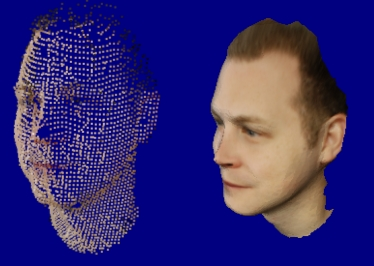
\includegraphics[width=0.46\textwidth]{pointCloud.jpg}
}
\hspace{5pt}
\subfigure{
	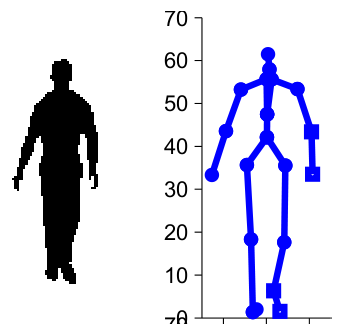
\includegraphics[width=0.3\textwidth]{mocapData.png}
}
\vspace{5pt}
\subfigure{
	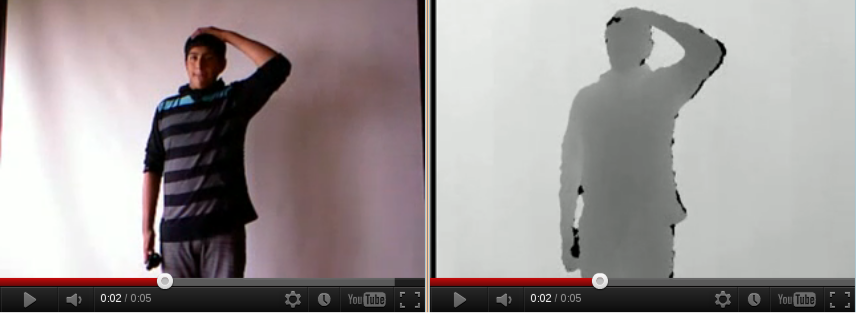
\includegraphics[width=0.7\textwidth]{kinectData.png}
}
\end{center}
\end{figure}
\end{frame}


\begin{frame}
\frametitle{Dimensionality reduction}
\centering
	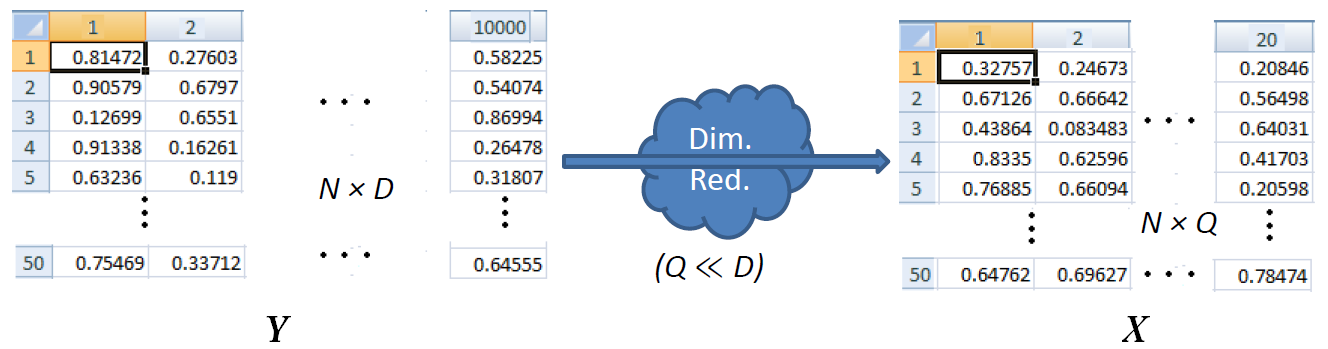
\includegraphics[width=1\textwidth]{dimReduction.png}
\end{frame}

\section{Dimensionality reduction techniques}
\begin{frame}
  \frametitle{Dimensionality reduction techniques 1/2}
    \alert{\Large{Probabilistic vs non-probabilistic}}\newline \newline
    	A probabilistic interpretation allows us to:
    	\begin{itemize}
    		\item Have a model of the data
    		\item Handle incomplete data
    		\item Generate/sample novel data
    		\item Extend the model with prior information or integrate it with other models (e.g. mixtures)
    	\end{itemize}
\end{frame}


\begin{frame}
\frametitle{Probabilistic, generative methods}
\begin{itemize}
\item \alert{Observed} (high-dimensional) data: $Y \in \mathbb{R}^{N \times D}$ \\
\emph{These contain redundant information}
\vspace{6pt}
\item \alert{Actual} (low-dimensional) data: \; \; $X \in \mathbb{R}^{N \times Q}, \; Q \ll D$
\emph{These are \underline{unobserved} and (ideally) contain only the minimum amount of information needed to correctly describe
 the phenomenon}
%	\end{align*}
\vspace{6pt}
\item Work ``backwards'': learn $f: X \mapsto Y$
\vspace{6pt}
\end{itemize}
\end{frame}

\begin{frame}
\frametitle{Probabilistic, generative methods}
\begin{itemize}
\item \alert{Model}:
	\begin{align*}
	y_{nd} &= f_d(\mathbf{x}_n, W)
					 + \epsilon_n \;, \;\;\; \epsilon_n \sim \mathcal{N}(0, \beta^{-1})\\
	\end{align*}
\item $p(Y|W,X,\beta)=\prod_{n=1}^N \mathcal{N}(\bfy_n|W\bfx_n, \beta^{-1}\mathbf{I})$ (\textit{linear case})
\item[]
\item $W,X \in \mathbb{R}^{N \times Q}$, $Q \ll D$
\item[]
\item $X$ is unobserved (\alert{latent space})

\end{itemize}
\end{frame}


\subsection{From Dual PPCA to GP-LVM}
\begin{frame}
\frametitle{From dual PPCA to GP-LVM}
\begin{itemize}
    \item \alert{PPCA} places a prior on and marginalises the latent space $X$ and optimises the \emph{linear} mapping's parameters $W$
    \item \alert{Dual PPCA} does the opposite: the prior is placed on the mapping parameters.
  \begin{columns}
   \column{0.5\textwidth}
        \begin{figure}
	\begin{center}
	      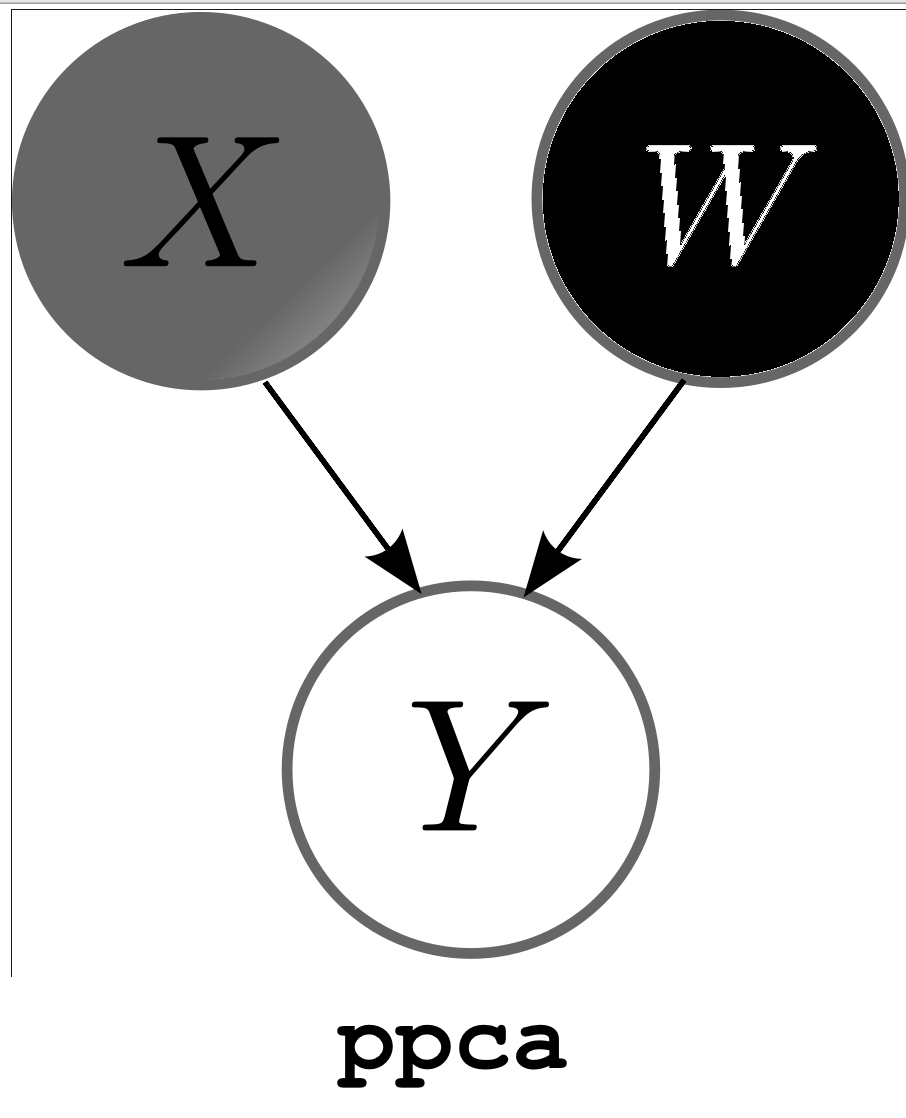
\includegraphics[width=0.4\textwidth]{ppcaSimple2.png}
	\end{center}
	\end{figure}
	\centering
	$p(Y|W,\beta)=\int p(Y|X,W,\beta)p(X) \intd X$
    
    
	\column{0.5\textwidth}
	\begin{figure}
	\begin{center}
	     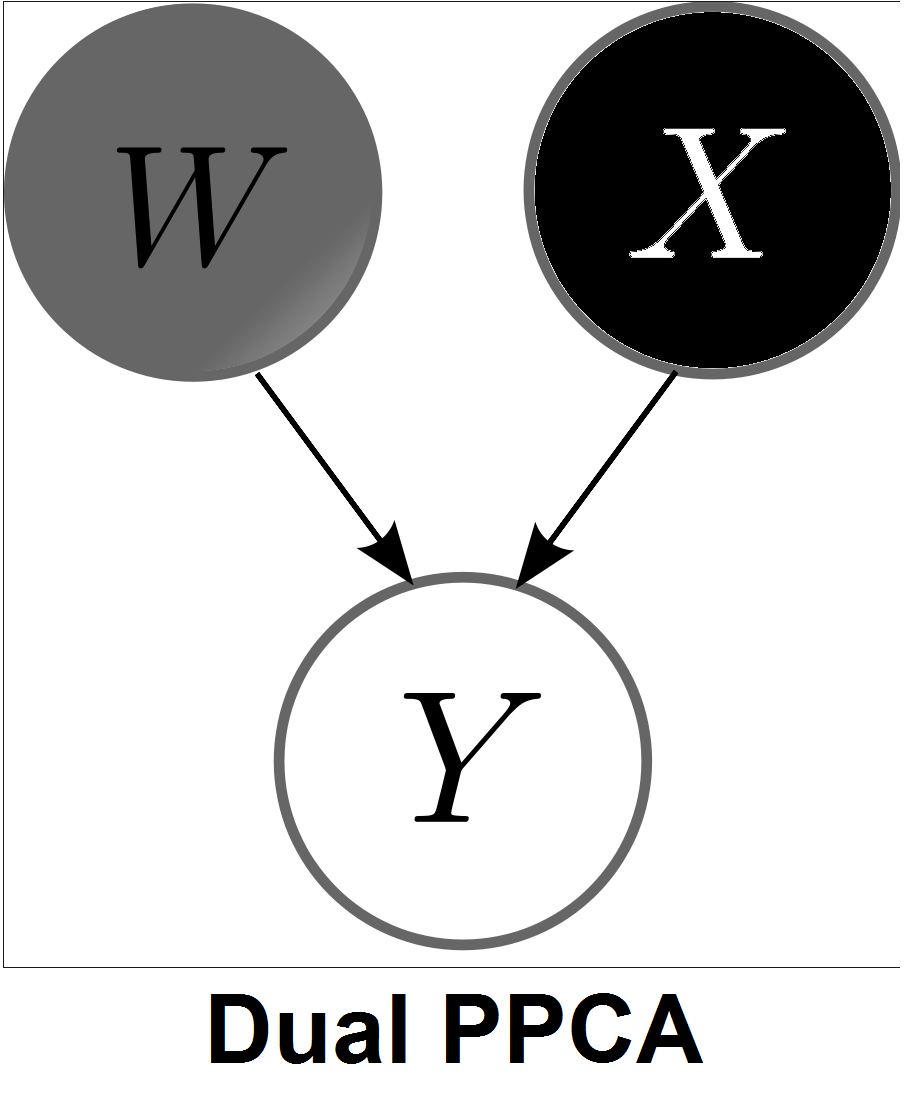
\includegraphics[width=0.4\textwidth]{gplvmSimple2.png}
	\end{center}
	\end{figure}
	\centering
	$p(Y|X,\beta)=\int p(Y|X,W,\beta)p(W) \intd W$
  

   \end{columns}
\end{itemize}
\end{frame}



\begin{frame}
\begin{itemize}
\frametitle{Gaussian process latent variable model (GP-LVM)}
\item<1-> \alert{PPCA} and \alert{Dual PPCA} are equivalent (equivalent eigenvalue problems for ML solution)
\item<1->[]
\item<2-> \alert{GP-LVM}: Instead of placing a prior $p(W)$ on the parametric mapping's parameters, we can place a prior directly
on the mapping function $\Rightarrow$ GP prior
\item<2->[]
\item<3-> A \alert{GP prior} $f \sim \mathcal{GP}(\bfzero, k(x,x'))$  allows for \emph{non-linear mappings}
    if the kernel $k$ is non-linear. For example:
          \begin{align*}
      \mathit{k_f} \left( \mathbf{x}_i, \mathbf{x}_j \right) = {} &  
		\sigma^2 \exp \left(
			- \frac{1}{2} \sum_{q=1}^{Q}  w_q \left(
                          \mathit{x_{i,q} - x_{j,q}} \right) ^2  \right)
    \end{align*}
\begin{flushright}
\footnotesize{
[Lawrence 2005]
}
\end{flushright}
\end{itemize}
\end{frame}




\begin{frame}
  \frametitle{Dimensionality reduction: Linear vs non-linear}    	
      \begin{figure}[t!]
        \centering
        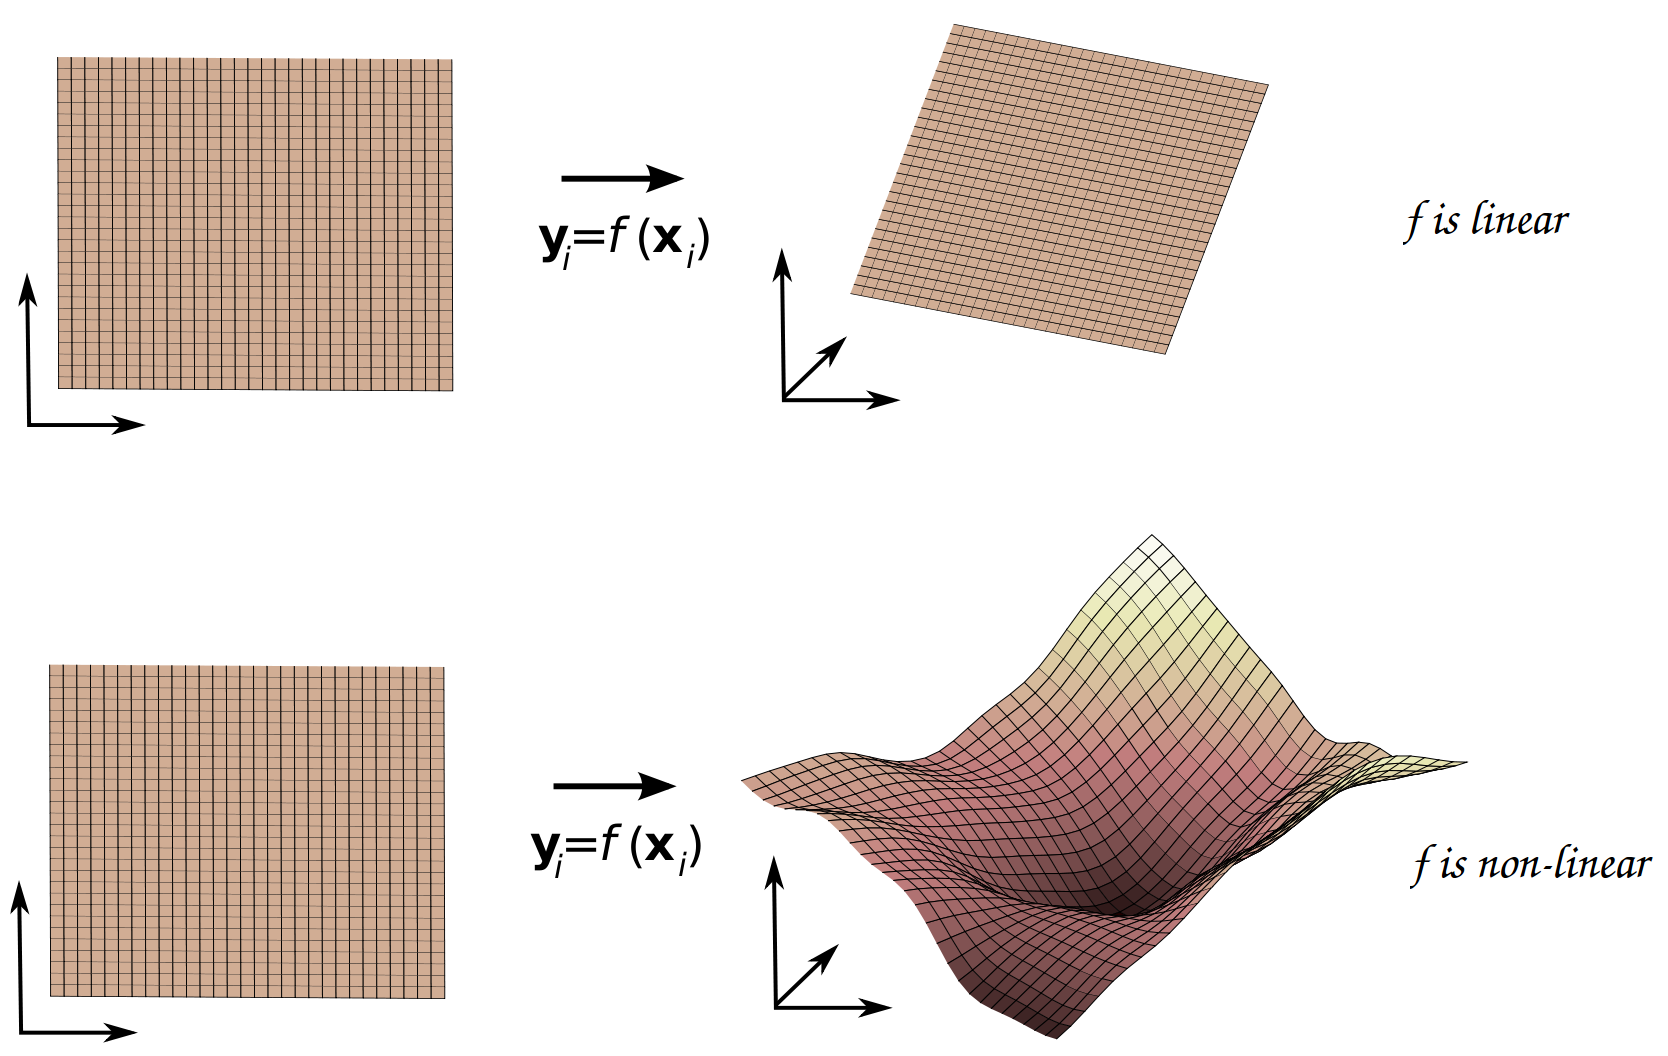
\includegraphics[width=0.9\textwidth]{linearVsNonlinear.png}
      \end{figure}
\begin{flushright}
\tiny{
\textit{Image from: ''Dimensionality Reduction the Probabilistic Way'', N. Lawrence, ICML tutorial 2008}
}
\end{flushright}
\end{frame}

% \begin{frame}
% \begin{itemize}
%     \item<1-> Probabilistic vs non-probabilistic
%       \begin{itemize}
% 	  \item Non-probabilistic, spectral approaches: PCA, isomap, ...
% 	  \item Probabilistic approaches: PPCA, GTM, GP-LVM, ...
%       \end{itemize}
% \vspace{7pt}
%     \item<2-> Probabilistic approaches are able to:
%       \begin{itemize}
% 	 \item Deal with missing data
% 	 \item Generate / sample new datapoints
% 	 \item Integrate with other models and extend
%       \end{itemize}
%     \end{itemize}
% \end{frame}




\begin{frame}
\frametitle{Optimising the GP-LVM}
\begin{columns}
 \column{0.25\textwidth}
 \only<1-2>{
 	\begin{figure}
	\begin{center}
	     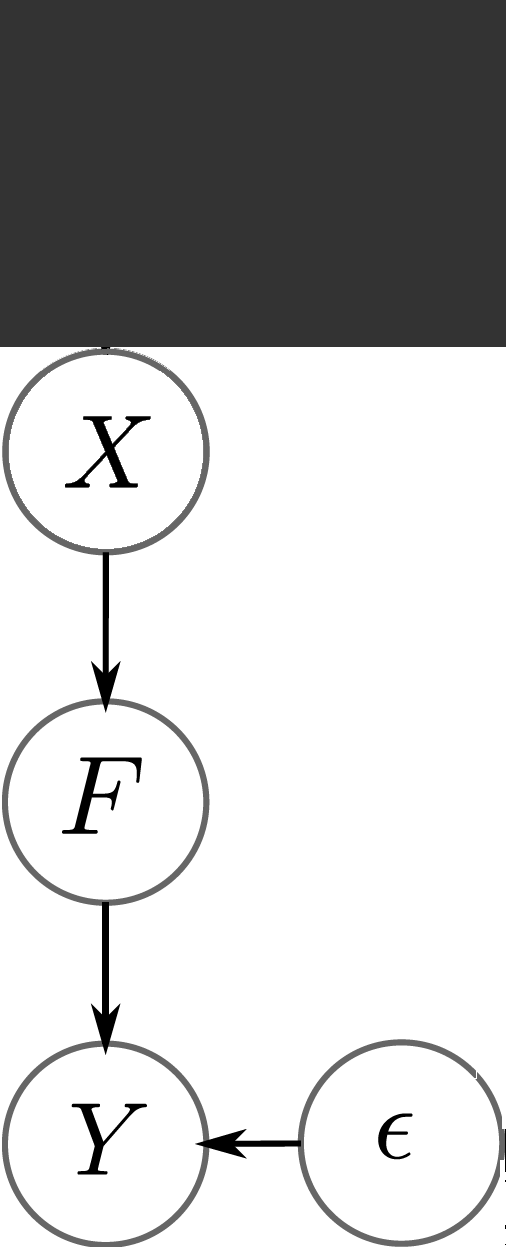
\includegraphics[width=1\textwidth]{gplvm.png}
	\end{center}
	\end{figure}
	}
	 \only<3->{
 	\begin{figure}
	\begin{center}
	     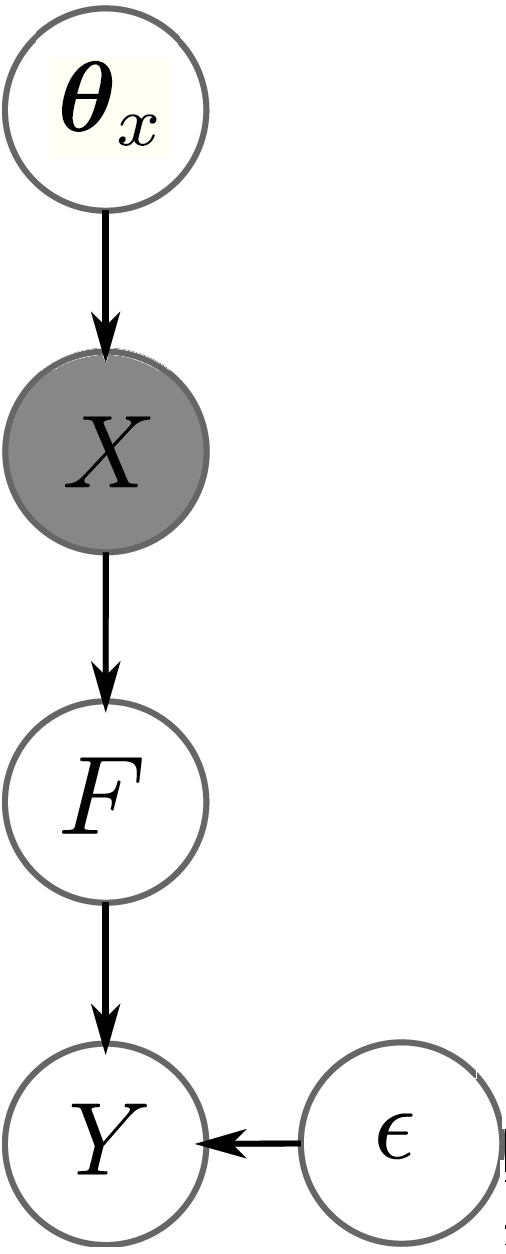
\includegraphics[width=1\textwidth]{bgplvm1.png}
	\end{center}
	\end{figure}
	}
 \column{0.8\textwidth}
 \hspace{-20pt}
 \begin{itemize}
                 \item<1-> Objective function for optimisation is $p(Y|X)$ \small{(found analytically, as $F$ is finite)}
	\vspace{5pt} \item<2-> Problem: this finds a single point (\alert{MAP}) estimate for $X$
	\vspace{5pt} \item<3-> We would prefer to instead find a \emph{distribution} over $X$ $\Rightarrow$ \emph{\alert{Bayesian} GP-LVM}
	\vspace{5pt} \item<4-> This allows for:
	\begin{itemize} 
	   \item training robust to overfitting 
	   \item automatic detection for the dimensionality of $X$
	   \item incorporating known structure on the latent space
	\end{itemize}
 \end{itemize}
\end{columns}
\end{frame}



\section{Bayesian GP-LVM}
\begin{frame}
 \frametitle{Bayesian GPLVM}
\begin{itemize}	
%\item Dataset: 
%	$$
%	Y \in R^{D} , X \in 
%	$$
\item
	GPLVM \alert{objective function}: 
	$$
	p(Y|X) = \int p \left( Y | \bff \right)	p(\bff | X) d \bff = \mathcal{N}(Y | \mathbf{0}, K_{NN}+\beta^{-1} I_N)
	$$
	The GPLVM is trained by maximizing $p(Y|X)$ w.r.t the mapping's parameters and $X$ (jointly) $\Rightarrow$ \textit{MAP} estimate,
\vspace{8pt}
\item \alert{Bayesian GPLVM}:
	Also integrate out $X$'s:
	$$
	p(Y) = \int p \left( Y | X \right) p(X) dX 
	$$ $$
	p(X) = \prod_{n=1}^{N} N(\bfx_n | \mathbf{0}, I_Q)
	$$
\vspace{8pt}
\pause
\item \alert{Tractability}:
	The marginal likelihood as well as the posterior $p(X | Y)$ are intractable
	    $\Rightarrow$ the variational framework of \small{[Titsias and Lawrence, 2010]} resolves this
\end{itemize}
\end{frame}



\begin{frame}
 \frametitle{Automatic dimensionality detection}
 \begin{itemize}
  \item Achieved by employing \emph{automatic relevance determination (ARD)} priors for the mapping $f$.
     \vspace{5pt}
  \item  $f \sim \mathcal{GP}(\bfzero, k_f)$ with:
      \begin{align*}
      \mathit{k_f} \left( \mathbf{x}_i, \mathbf{x}_j \right) = {} &  
		\sigma^2 e^{
			- \frac{1}{2} \sum_{q=1}^{Q}  w_q \left(
                          \mathit{x_{i,q} - x_{j,q}} \right) ^2 }
    \end{align*}
 \item Example:
    \begin{figure}
    \begin{center}
    \subfigure{
	  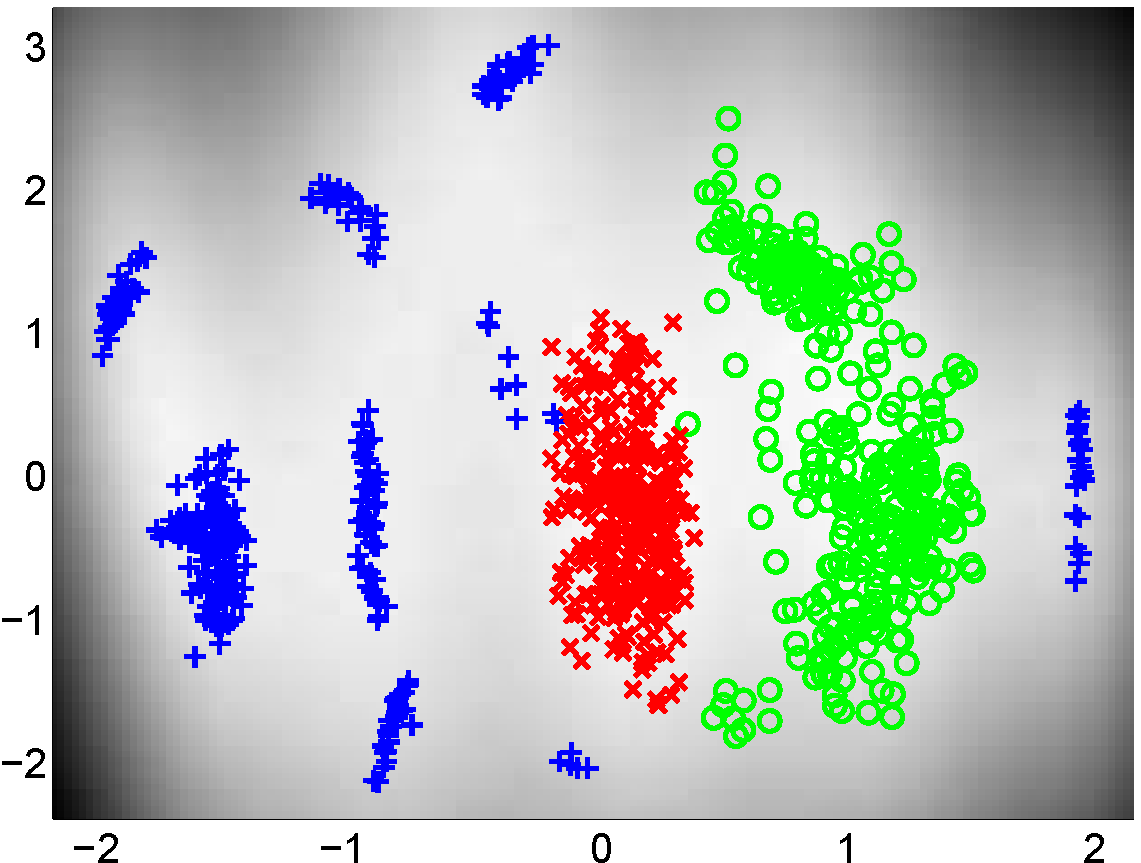
\includegraphics[width=0.43\textwidth]{demOilVargplvm1}
    }
    \hspace{5pt}
    \subfigure{
	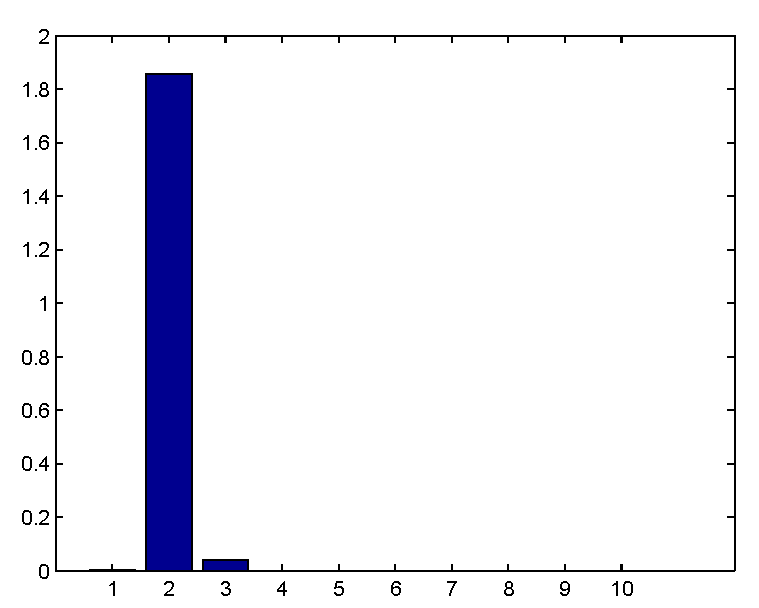
\includegraphics[width=0.4\textwidth]{demOilVargplvm1Scales}
    }
    \end{center}
    \end{figure}
\end{itemize}
\end{frame}


\section{Structure in the latent space}
\subsection{Modelling dynamics}
\begin{frame}
	\frametitle{Modelling dynamics}
 \begin{columns}
    \column{0.2\textwidth}
      \begin{figure}
      \begin{center}
	  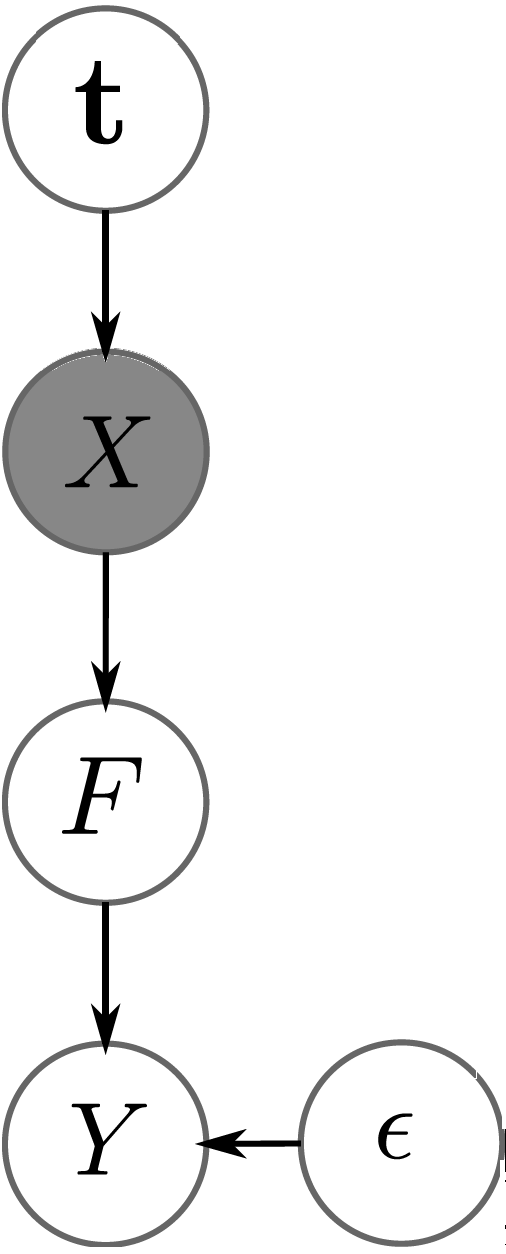
\includegraphics[width=1\textwidth]{bgplvm1b.png}
    \end{center}
    \end{figure}
 \column{0.9\textwidth}
 
\begin{itemize}
  \item<1-> If $Y$ form is a \alert{multivariate time-series}, then $X$ also has to be one
  \vspace{5pt}
  \item<2-> Place a \alert{temporal GP prior} on the latent space: 
    $\bfx = x(t) = \mathcal{GP}(\bfzero, k_x)$
\vspace{5pt}
  \item<3-> Dynamics are encoded in the covariance matrix $K_x = k_x(\bft,\bft)$,
     e.g. forcing $K_x$ to be block-diagonal allows to jointly model individual sequences
\vspace{5pt}
 \item<4-> \emph{Video examples...}
\end{itemize}

\end{columns}
\begin{flushright}
\small{
[Damianou et al., 2011]
}
\end{flushright}
\end{frame}


\begin{frame}
\frametitle{Modelling sequences}
\begin{itemize}
   \item  
     Dynamics are encoded in the covariance matrix $K_x = k_x(\bft,\bft)$,
     e.g. forcing $K_x$ to be block-diagonal allows to jointly model individual sequences
    \begin{figure}
    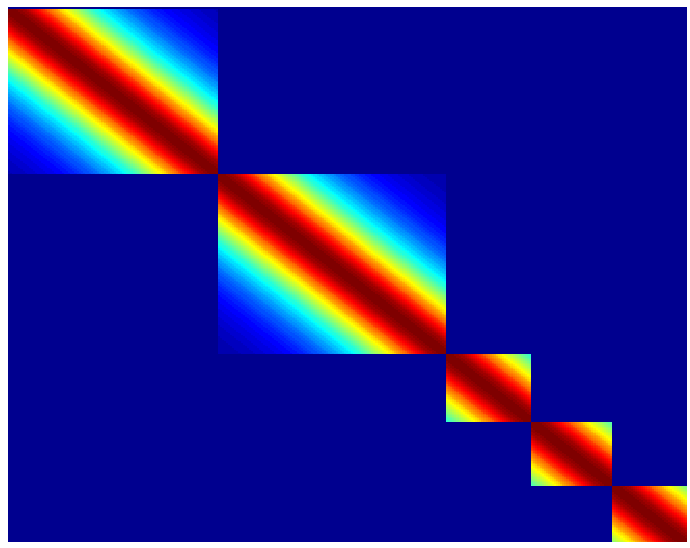
\includegraphics[width=0.4\textwidth]{blockDiagonalCov}
    \end{figure}
\end{itemize}
\end{frame}


\subsection{Multi-modal modelling}
\begin{frame}
	\frametitle{Multi-modal modelling}
    \begin{itemize}
       \item Several observation modalities for the same underlying phenomenon
        \vspace{3pt}
      \item \alert{Challenge}: factorise the latent space into parts that are either private or shared for all modalities
       \vspace{3pt}
     \item \alert{Bayesian solution}: use a separate set of \emph{ARD} parameters for each modality
        \vspace{3pt}
    \item The ARD weights are optimised to learn the responsibility of each latent dimension for generating each of the observation spaces
    \end{itemize}
      \begin{figure}
      \begin{center}
	  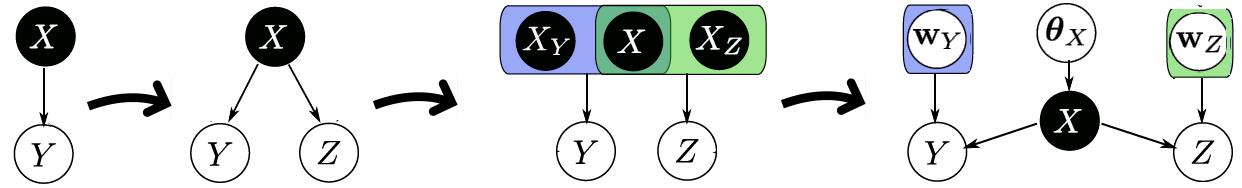
\includegraphics[width=1.05\textwidth]{graphicalmodel.png}
    \end{center}
    \end{figure}
\end{frame}

\begin{frame}
\frametitle{Manifold Relevance Determination}
\begin{itemize}
\item The high-level description of the model:
\begin{figure}
\begin{center}
{
        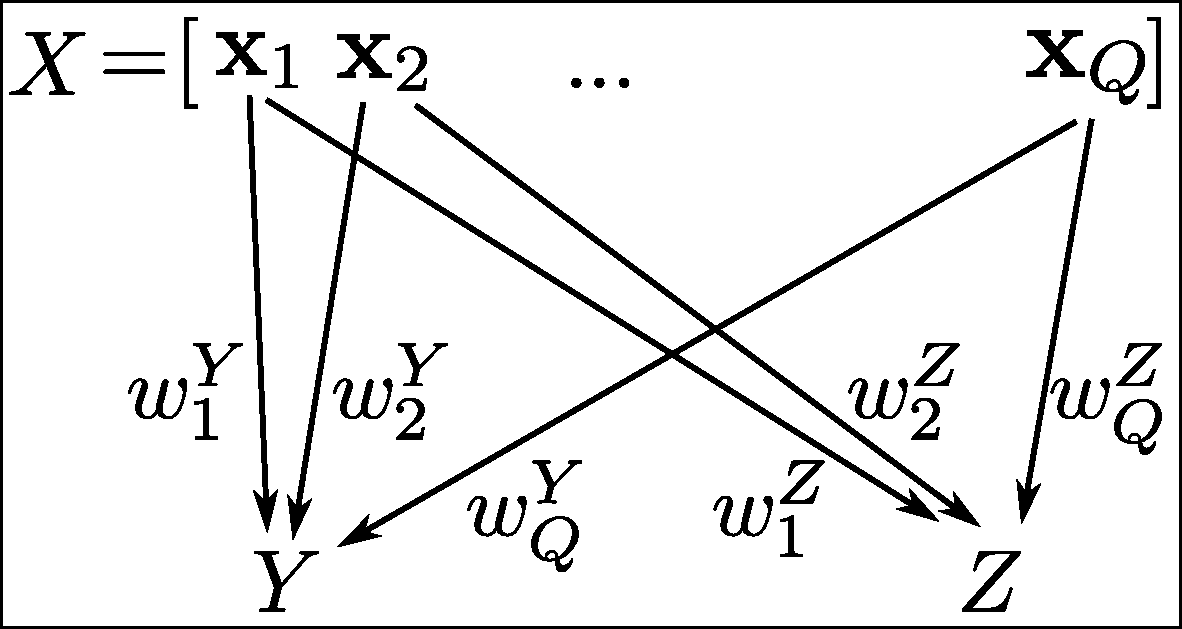
\includegraphics[width=0.73\textwidth]{modelWeights}
}
\end{center}
\end{figure}

\item Bayesian optimisation ensures that irrelevant dimensions will be assigned a zero weight
\end{itemize}
\begin{flushright}
\small{
[Damianou et al., 2012]
}
\end{flushright}
\end{frame}


\begin{frame}
\frametitle{Example: Yale faces}
\begin{figure}
\movie{
\includegraphics[width=.95\textwidth]{movieFrame.jpg}}{YaleDataset.avi}
\end{figure}
\begin{itemize}
	\item Dataset $Y$: $3$ persons under all illumination conditions
	\item Dataset $Z$: As above for $3$ different persons
	\item Align datapoints $\bfy_n$ and $\bfz_n$ only based on the lighting direction
\end{itemize}
%\includemovie[options]{67.7pt}{36.4pt}{yaleDataset.avi} %% 677, 364
%\href{run:yaleDataset.swf}
   % \begin{figure}
    %\includemovie[scale=0.5]{yaleDataset.swf}
    %\end{figure}
\end{frame}



\begin{frame}
\frametitle{Results}
\begin{itemize}
  \item Latent space $X$  initialised with $14$ dimensions
  \item Weights define a segmentation of $X$
\begin{figure}
\begin{center}
{
        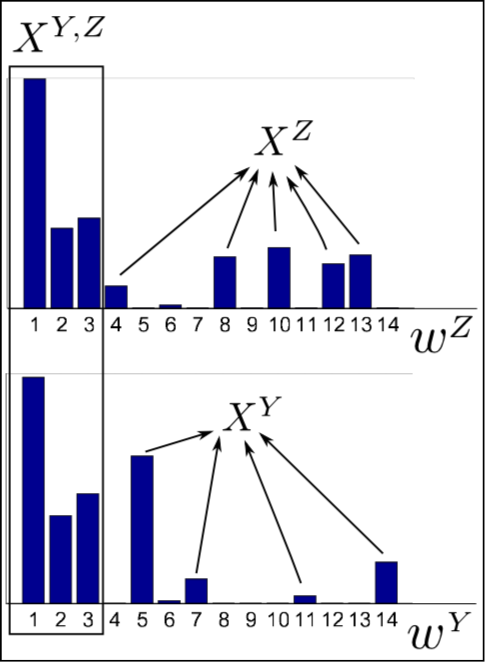
\includegraphics[width=0.43\textwidth]{yaleScales.png}
}
\end{center}
\end{figure}
\item Video...
\end{itemize}
\end{frame}


\begin{frame}
	\frametitle{Summary}
	\begin{itemize}
		             \item \alert{GP-LVM}: probabilistic non-linear dimensionality reduction
		\vspace{6pt} \item \alert{Bayesian GP-LVM}: placing a prior over and marginalising the latent space
		\vspace{6pt} \item \alert{Dynamical framework}: constraining the latent space to be a timeseries
		\vspace{6pt} \item \alert{Multi-modal framework}: automatically segment the latent space to shared and private subspaces
	\end{itemize}
\end{frame}

\begin{frame}
 \frametitle{Thanks}
   \begin{columns}
    \column{0.33\textwidth}    
    \begin{block}{KTH}
      Carl Henrik Ek
    \end{block}

    \column{0.33\textwidth}
    \begin{block}{Univ. of Oxford}
      Michalis Titsias
    \end{block}
    
    \column{0.33\textwidth}
    \begin{block}{Univ. of Sheffield}
      Neil Lawrence
    \end{block}
  \end{columns}
  \vspace{1cm}
  \begin{block}{Funding}
    \begin{itemize}
    \item University of Sheffield Moody endowment fund
    \item Greek State Scholarships Foundation (IKY)
    \end{itemize}
  \end{block}

\end{frame}

%
%\begin{frame}
%	\frametitle{}
%	\begin{block}{eQTL mapping}
%          Expression quantitative trait loci (eQTL) mapping is a statistical technique with the goal to identify causal associations 
%          between variable genetic loci and the expression levels of individual genes.
%	\end{block}
%\end{frame}
%
%
%
%\begin{frame}
%  \frametitle{Standard testing approaches}
%  \begin{itemize}
%    \item Traditional association mapping for a single phenotypic
%      trait 
%     \begin{itemize}
%     \item \alert{Independent linear models} mapping from SNPs to phenotype  
%     \end{itemize}
%     \only<1->
%     {
%       {\small
%         \begin{align*}
%           y_{j} = \underbrace{b_{n}\left(\theta_{n}
%               s_{n,j}\right)}_\mathrm{genetic} \,\, + \,\, \underbrace{\psi_{j,n}}_{\text{noise}}
%        \end{align*} 
%      }
%    }
%  \item<3-> For example, assuming Gaussian observation noise --
%    likelihood ratio 
%    statistics can serve as a means of statistical testing 
%    \begin{align*}
%      a &= b \nonumber \\
%      b &= c
%    \end{align*}    
%\end{itemize}
%\end{frame}
%
%
%\begin{frame}
%  \frametitle{Confounding factors}
%  \begin{columns}
%    \column{0.6\textwidth}
%    \begin{itemize}
%    \item<1-> Introduce correlation between samples
%    \item<2-> If the factors are {\color{mediumGreen} known} it's
%      possible to correct for them
%    \item<4-> If the factors are {\color{mediumRed} unknown}, they need to be estimated
%      from the gene expression data
%    \end{itemize}
%    
%    \column{0.4\textwidth}
%    \only<1>{
%      \begin{figure}[t!]
%        \centering
%        \includegraphics[width=0.8\textwidth]{temp.png}
%      \end{figure}
%    }
%    \only<2>{
%      \begin{figure}[t!]
%        \centering
%        \includegraphics[width=0.8\textwidth]{temp.png}
%      \end{figure}
%    }
%  \end{columns}
%\end{frame}
%
%
%
%
%
%\begin{frame}
%  \frametitle{}
%  \begin{center}
%    \Huge PANAMA\pause\\
%    \vspace{0.5cm}
%    \large Probabilistic ANAlysis of genoMic dAta
%  \end{center}
%\end{frame}
%
%\begin{frame}
%  \frametitle{}
%  \begin{figure}[t!]
%    \centering
%    \includegraphics[width=0.6\textwidth]{temp.png}
%  \end{figure}
%\end{frame}
%
%\begin{frame}
%  \frametitle{PANAMA}
%  \framesubtitle{Learning a dictionary of confounders}
%  \begin{figure}[t!]
%    \centering
%    \includegraphics[width=0.8\textwidth]{temp.png}
%  \end{figure}
%  \begin{itemize}
%  \item we put a Gaussian prior on $\mathbf{W}$ and integrate out the
%    weights \pause
%  \item related to PCA/FA \pause
%  \item allow for an individual weighting of the latent variables
%  \end{itemize}
%\end{frame}
%
%
%
%
%
%
%\begin{frame}
%  \frametitle{Evaluation on yeast}
%  \begin{center}
%  \includegraphics[width=0.9\textwidth]{temp}
%  \end{center}
%  \begin{flushright}
%    [Smith et al., 2008]
%  \end{flushright}
%\end{frame}
%
%
%\begin{frame}
%\frametitle{Comparison to the other models}
%\begin{table}[h!]
%  \centering
%  \begin{tabular}{lccc}
%    \toprule
%    & Low rank & Confounders & Preserves genetic signal \\
%    \midrule
%    SVA & \checkmark & \checkmark & \checkmark (partially)\\
%    PEER & \checkmark & \checkmark & \checkmark (partially)\\
%    ICE &  & \checkmark &   \\
%    %LMM-EH &  & \checkmark & \\
%    \textbf{PANAMA} & \checkmark & \checkmark & \checkmark  \\
%    LINEAR &  &  & \checkmark \\
%    \bottomrule
%  \end{tabular}
%\end{table}
%\end{frame}
%
%
%\begin{frame}
%   \begin{columns}
%    \column{0.50\textwidth}    
%    \begin{block}{MPI T\"ubingen}
%      Oliver Stegle
%    \end{block}
%
%    \column{0.50\textwidth}
%    \frametitle{Thanks}
%    \begin{block}{University of Sheffield}
%      Neil Lawrence
%    \end{block}
%  \end{columns}
%  \vspace{1cm}
%  \begin{block}{Funding}
%    \begin{itemize}
%    \item EPSRC
%    \item FP7 PASCAL II Network of Excellence
%    \item Amazon AWS
%    \end{itemize}
%  \end{block}
%
%\end{frame}

\end{document}
